\documentclass{../source/Experiment}

\major{信息工程}
\name{姚桂涛}
\title{形态学和其他集合运算}
\stuid{3190105597}
\college{信息与电子工程学院}
\date{\today}
\lab{}
\course{数字图像处理}
\instructor{李东晓}
\grades{}
\expname{形态学和其他集合运算}
\exptype{设计验证}
\partner{}
\begin{document}
    \makecover
    \section{实验任务}

        本次选择的是PROJECT-06-01题目。

        \begin{enumerate}
            \item 编写一个程序实现二值膨胀和腐蚀,可以用3 x 3的任意结构元素。
            \item 编写一个程序,实现集合交集、差集和补集运算。
        \end{enumerate}

    \section{算法设计}

        为了视觉效果,实验中是对黑色元素进行处理,即把黑色看成1,白色看成0。
        
        二值膨胀和腐蚀程序中,结构元素为$3\times3$的矩形,原点位于中心点,采用了移动结构元素并判断的方式进行运算。

        交集差集补集程序中直接使用了矩阵运算实现。

    \section{代码实现}
        本次实验编程语言选择的是Matlab。

        二值膨胀程序如下:
        \lstinputlisting[
            language  =   matlab
            ]{第四次/my_dilation.m}

        二值腐蚀程序如下:
        \lstinputlisting[
            language  =   matlab
            ]{第四次/my_erosion.m}


        集合运算程序如下:
        \lstinputlisting[
            language  =   matlab
            ]{第四次/set_cal.m}

        主程序如下:

        \lstinputlisting[
            language  =   matlab
            ]{第四次/main.m}

    \section{实验结果}
        实验结果如下:

        \begin{figure}[H]
            \centering
            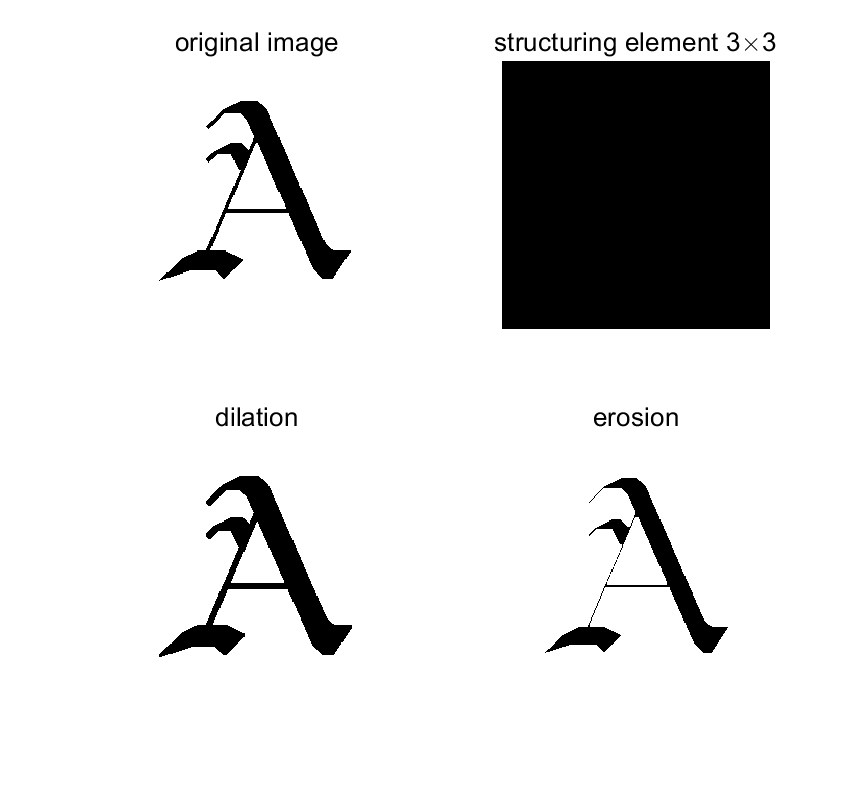
\includegraphics[width = 0.6\textwidth]{第四次/f1.png}
            \caption{二值腐蚀和膨胀实验结果}
        \end{figure}

        \begin{figure}[H]
            \centering
            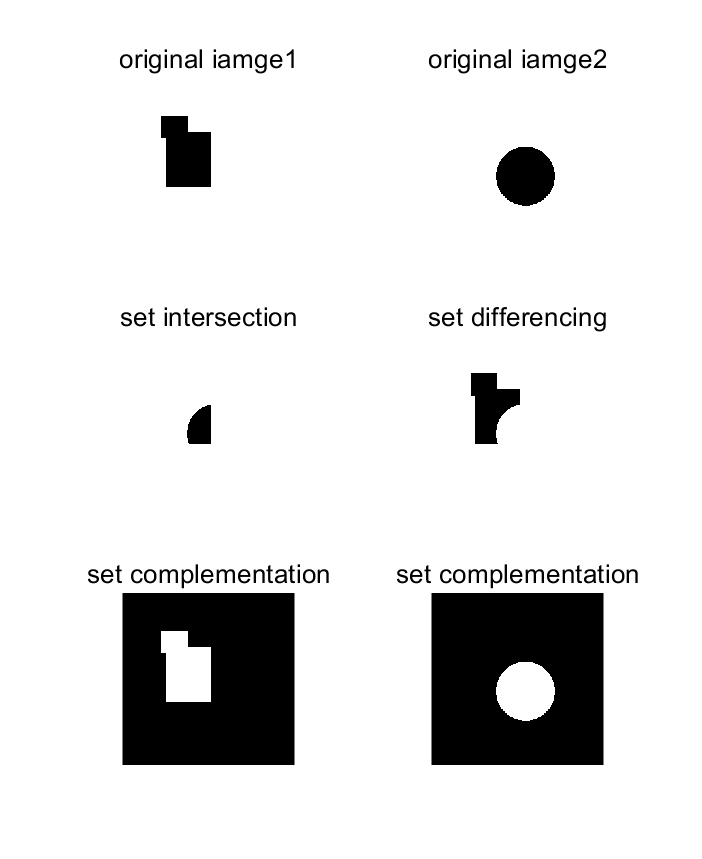
\includegraphics[width = 0.6\textwidth]{第四次/f2.png}
            \caption{集合运算实验结果}
        \end{figure}

    \section{总结}
    本次实验主要是通过Matlab编程语言实现了课程中所讲过的形态学和其他集合运算。
    
    一开始实验是直接对于白色元素进行处理的,但是效果并不是很好,所以最好换成了对黑色元素进行处理。

\end{document}



